\section{Methodik, @Tobias Krug}
\subsection{Schemata}
\subsection{Automatisierung}
\subsection{Ausführungsumgebungen für Tests}

\section{Analyse \& Diskussion, @Till Huelder}
\subsection{Vergleich der Schemata}
\subsection{Vergleich der Ausführungsumgebungen}

\section{Thesen, @Tobias Klama}

Der folgende Abschnitt behandelt Thesen bezüglich der Zusammenhänge zwischen Messgrößen und Parametern.
Die Thesen werden anhand der Messergebnisse, der zugrunde liegenden Schema-Architektur und Hardware erörtert.

\subsection{Es besteht eine Korrelation von RAM mit world\_size}

Wie zu erwarten steigt der summierte RAM-Bedarf über alle Processors mit steigender world\_size
(Fig \ref{fig:hpcAsumRSSsmall}-l, Fig \ref{fig:NUCsumRSSsmall}-l, Fig \ref{fig:hpcAsumRSSnormal}-l und Fig \ref{fig:NUCsumRSSnormal}-l).
Insbesondere bei Schema 1 und 3 liegt jedem Processor
die gesamte Datenmenge an Parametern und P-Matrix im Arbeitsspeicher vor.
Schema 2 teilt die P-Matrix in Blöcke auf und scattert diese an alle ranks.
Diese Aufteilung und dadurch, dass rank\_0 auch an sich selbst
scattert führt dazu, dass rank\_0 von Schema 2 einen höheren RAM Bedarf hat als bei Schema 1 und 3.
Weiterhin kann den Messungen entnommen werden,
dass ab einer world\_size von 4 der gesamt benötigte RAM Bedarf von Schema 2 niedriger als bei den anderen beiden Schemas ist und darüber
hinaus langsamer ansteigt.
Das liegt daran, dass jeder rank nur einen Bruchteil entsprechend der world\_size der Daten erhält und somit jede Vergrößerung der
world\_size einen niedrigeren durchschnittlichen RAM Bedarf ergibt.
In Fig \ref{fig:hpcAmaxRSSsmall}-l, Fig \ref{fig:NUCmaxRSSsmall}-l, Fig \ref{fig:hpcAmaxRSSnormal}-l und Fig \ref{fig:NUCmaxRSSnormal}-l
ist der maximal benötigte RAM-Bedarf von rank\_0 in jedem Schema dargestellt.
Der Bedarf bleibt über alle world\_sizes konstant, da jeder rank\_0
unabhängig von Schema und world\_size die gesamte Datenmenge im Arbeitsspeicher vorliegen hat.

\subsection{Es besteht eine Korrelation runtime mit com\_interval}

Das com\_interval ist der Parameter, der angibt wie oft Ranks miteinander kommunizieren.
Anhand der Diagramme Fig \ref{fig:hpcAcomTimesmall}-f, Fig \ref{fig:NUCcomTimesmall}-f, Fig \ref{fig:hpcAcomTimenormal}-f
und Fig \ref{fig:NUCcomTimenormal}-f
ist eine klare Korrelation zwischen der benötigten runtime zur Konvergenz und com\_interval erkennbar. Zur Darstellung eines
eindeutigeren Verlaufs sind Messungen mit einer höheren com\_interval-Auflösung in Fig \ref{fig:ScatRunCom} und \ref{fig:ScatStepCom}
dargestellt. Die runtime ist bei allen drei Schemas sehr ähnlich und die Iterationsanzahl sogar meist identisch,
daher überdecken die Messpunkte von Schema 3 zum Großteil die anderen beiden Schemas. Die beiden nebeneinander verlaufenden Kurven resultieren
aus den zwei unterschiedlichen world\_sizes 2 \& 4. In Fig \ref{fig:ScatRunCom} gehört die Kurve mit niedrigerer runtime zu world\_size 4 und
in Fig \ref{fig:ScatStepCom} gehört der Verlauf mit höherer benötigter Iterationsanzahl zu world\_size 4.
Eine durch niedriges com\_interval geringere Häufigkeit der Kommunikation zwischen den Processors führt dazu, dass die Processors
mehr Iterationen der Value Iteration durchführen bevor die Ergebnisse untereinander ausgetauscht werden.
Im Idealfall würde durch selteneres Austauschen weniger Zeit für eben diese Kommunikation verwandt werden und die runtime dadurch sinken.
Jedoch im Gegensazt dazu führt ein größeres com\_interval dazu, dass durch das seltenere
Update des J-Vektors die Konvergenz beinträchtigt wird. Das führt zu einer höheren benötigten Iterationsanzahl was schlussendlich
wieder zu einer höheren Anzahl an benötigten Kommunikationen und dadurch
zu einer längeren Laufzeit führt. Der ansteigende Bedarf an Iterationen bei steigendem com\_interval ist in Fig \ref{fig:ScatStepCom}
dargestellt.
Für die dargestellten NUC-Messungen haben diese beiden sich gegensätzlichen Effekte in Summe bei com\_interval 3 ihr Minimum.
Bei den anderen Targets liegt das Minimum ebenfalls in dieser Größenordnung. Ohne explizite Messung mit com\_interval 3 kann jedoch
kein Schluss daraus gezogen werden ob das Minimum bei com\_interval 3 hardware-unabhängig ist.

\begin{figure}[h]
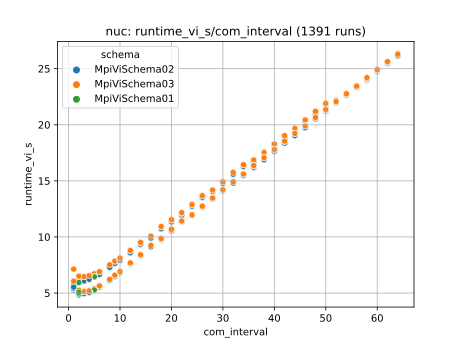
\includegraphics[width=0.5\textwidth]{./gen/img/nuc/small/scatterplot_com_interval_runtime_vi_s.pdf}
\caption{NUC, runtime vs. com\_interval, world\_size 2 \& 4}
\label{fig:ScatRunCom}
\end{figure}

\begin{figure}[h]
\includegraphics[width=0.5\textwidth]{./gen/img/nuc/small/scatterplot_com_interval_steps_total.pdf}
\caption{NUC, runtime vs. com\_interval, world\_size 2 \& 4}
\label{fig:ScatStepCom}
\end{figure}

\subsection{Es besteht eine inverse Korrelation zwischen world\_size und runtime}

Eine größere world\_size sorgt für eine größere Anzahl an Berechnungen, die parallel durchgeführt werden.
Sind die Berechnungen pro Processor komplex/lange genug um den Mehraufwand an inter-Processor Kommunikation zu
gerechtfertigen so führt das zu einer veringerten runtime.
In der vorliegenden Value-Iteration ist der Effekt nicht besonders stark, da die Berechnungen für die nötige
Konvergenz nicht unabhängig voneinander durchgeführt werden können. Ein Austausch der Ergebnisse während des Algorithmus ist für ein
richtiges Ergebnis zwingend nötig. Das führt zu einer notwendigen Kommunikation zwischen den Processors,
die dem Effekt der Zeitersparnis durch Parallelisierung entgegenwirkt.
Anhand der Messergebnisse in Fig \ref{fig:hpcAworldTimenormal}-c und Fig \ref{fig:NUCworldTimenormal}-c kann besonders beim normalen Datensatz
kein eindeutiger Zusammenhang zwischen der world\_size und der runtime festgestellt werden.
Die Auswirkung einer größeren world\_size fällt von Target zu Target unterschiedlich aus.
Bei den isolierten Targets NUC, RPi und Local bleibt die Zeit weitgehend gleich mit einer Tendenz zu geringfügig schnellere Ausführung
bei größerer world\_size. Aufgrund der Varianz der Messdaten ist es jedoch nicht möglich eine zuverlässige darüber zu treffen.
Beim kleinen Datensatz (siehe Fig \ref{fig:hpcAworldTimesmall}-c und Fig \ref{fig:NUCworldTimesmall}-c) ist im Allgemeinen,
bis auf world\_size 56 bei HPC Class mixed, eine leichte Tendenz zur schnelleren Ausführung bei größerer world\_size zu beobachten.
Das liegt vermutlich daran, dass die HPCs frei zugänglich sind und die Wahrscheinlichkeit weiterer Nutzer, die die runtime
stören, mit steigender world\_size und grundsätzlich längerer Berechnungsdauer beim größeren Datensatz steigt.
Weiterhin sind die Schemas mit blockierenden MPI-Funktionen implementiert. Das bedeutet, dass in jeder Kommunikations-Iteration
auf den langsamsten Processor gewartet wird. So führt einerseits die Heterogenität beim mixed-cluster zu Performance Einbußen,
weiterhin, falls ein Processor durch einen zusätzlichen Nuter am HPC verlangsamt wird müssen alle restlichen Processors warten.

Für eine eindeutige Aussage der genauen Korrelationen sind Messungen mit garantiert freiem Cluster und kontrollierten Störungen nötig.

\section{Beiträge}
- Testumgebung für automatisierte Analyse von Open MPI Kommunikationsschemata für asynchrone Value Iteration auf verschiedenen Ausführungsumgebungen
